% Generated by make_results_figures.py from media/data/*.json.
% Those numbers are DIGITIZED from the published figures, not the
% original data: see media/data/README.md.
\documentclass[border=6pt]{standalone}
\usepackage[T1]{fontenc}
\usepackage{helvet}
\renewcommand{\familydefault}{\sfdefault}
\usepackage{amsmath}
\usepackage{tikz}
\usetikzlibrary{arrows.meta,calc,decorations.pathreplacing}
\definecolor{spaceC}{HTML}{3B6EA5}
\definecolor{timeC}{HTML}{D9822B}
\definecolor{hcC}{HTML}{6B5B95}
\definecolor{vcC}{HTML}{8A7F72}
\definecolor{ink}{HTML}{2B2B2B}
\definecolor{muted}{HTML}{6B6B6B}
\definecolor{gridC}{HTML}{E6E4E0}
\definecolor{nanC}{HTML}{EFEDEA}
\definecolor{s1}{HTML}{2A78D6}
\definecolor{s2}{HTML}{EB6834}
\definecolor{s3}{HTML}{1BAF7A}
\definecolor{s4}{HTML}{EDA100}
\definecolor{s5}{HTML}{E87BA4}
\begin{document}
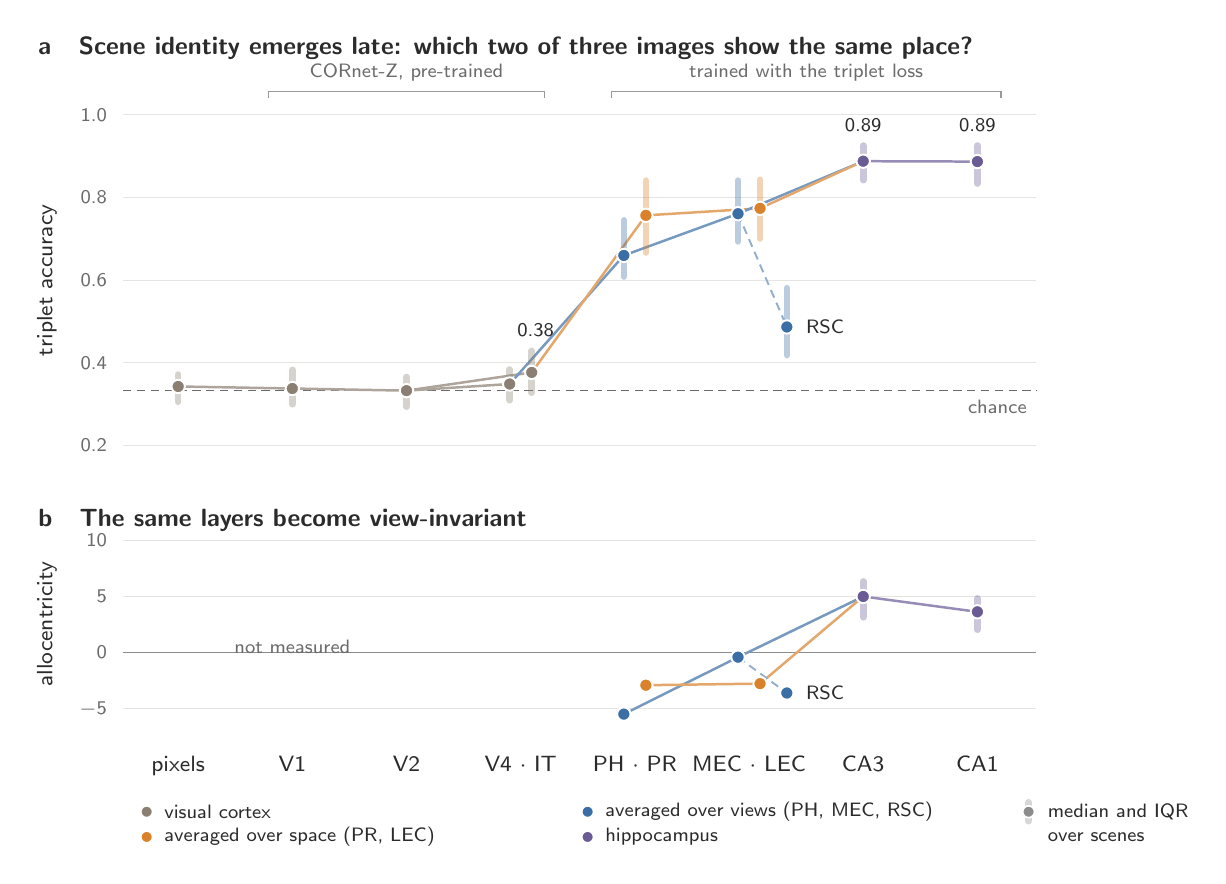
\begin{tikzpicture}[font=\footnotesize,
  tick/.style={font=\scriptsize,text=muted},
  lab/.style={font=\footnotesize,text=ink},
  ttl/.style={font=\small\bfseries,anchor=west,text=ink}]

\node[ttl] at (-1.2,8.75) {a\quad Scene identity emerges late: which two of three images show the same place?};
\draw[gridC,line width=0.4pt] (0.000,3.700)--(11.600,3.700);
\node[tick,anchor=east] at (-0.080,3.700) {0.2};
\draw[gridC,line width=0.4pt] (0.000,4.750)--(11.600,4.750);
\node[tick,anchor=east] at (-0.080,4.750) {0.4};
\draw[gridC,line width=0.4pt] (0.000,5.800)--(11.600,5.800);
\node[tick,anchor=east] at (-0.080,5.800) {0.6};
\draw[gridC,line width=0.4pt] (0.000,6.850)--(11.600,6.850);
\node[tick,anchor=east] at (-0.080,6.850) {0.8};
\draw[gridC,line width=0.4pt] (0.000,7.900)--(11.600,7.900);
\node[tick,anchor=east] at (-0.080,7.900) {1.0};
\node[lab,rotate=90,anchor=south] at (-0.720,5.800) {triplet accuracy};
\draw[muted,densely dashed,line width=0.5pt] (0,4.400)--(11.600,4.400);
\node[tick,anchor=north east] at (11.600,4.400) {chance};
\draw[vcC!70,line width=0.9pt] (0.700,4.451)--(2.150,4.425);
\draw[vcC!70,line width=0.9pt] (2.150,4.425)--(3.600,4.398);
\draw[vcC!70,line width=0.9pt] (3.600,4.398)--(4.910,4.482);
\draw[vcC!70,line width=0.9pt] (3.600,4.398)--(5.190,4.629);
\draw[spaceC!70,line width=0.9pt] (4.910,4.482)--(6.360,6.115);
\draw[timeC!70,line width=0.9pt] (5.190,4.629)--(6.640,6.624);
\draw[spaceC!70,line width=0.9pt] (6.360,6.115)--(7.810,6.645);
\draw[timeC!70,line width=0.9pt] (6.640,6.624)--(8.090,6.713);
\draw[spaceC!70,line width=0.9pt] (7.810,6.645)--(9.400,7.312);
\draw[timeC!70,line width=0.9pt] (8.090,6.713)--(9.400,7.312);
\draw[hcC!70,line width=0.9pt] (9.400,7.312)--(10.850,7.307);
\draw[spaceC!55,line width=0.7pt,densely dashed] (7.810,6.645)--(8.430,5.207);
\draw[vcC,line width=2.4pt,line cap=round,opacity=0.35] (0.700,4.256)--(0.700,4.603);
\filldraw[fill=vcC,draw=white,line width=0.7pt] (0.700,4.451) circle (0.085);
\draw[vcC,line width=2.4pt,line cap=round,opacity=0.35] (2.150,4.225)--(2.150,4.661);
\filldraw[fill=vcC,draw=white,line width=0.7pt] (2.150,4.425) circle (0.085);
\draw[vcC,line width=2.4pt,line cap=round,opacity=0.35] (3.600,4.194)--(3.600,4.572);
\filldraw[fill=vcC,draw=white,line width=0.7pt] (3.600,4.398) circle (0.085);
\draw[vcC,line width=2.4pt,line cap=round,opacity=0.35] (4.910,4.277)--(4.910,4.666);
\filldraw[fill=vcC,draw=white,line width=0.7pt] (4.910,4.482) circle (0.085);
\draw[vcC,line width=2.4pt,line cap=round,opacity=0.35] (5.190,4.372)--(5.190,4.902);
\filldraw[fill=vcC,draw=white,line width=0.7pt] (5.190,4.629) circle (0.085);
\draw[spaceC,line width=2.4pt,line cap=round,opacity=0.35] (6.360,5.847)--(6.360,6.561);
\filldraw[fill=spaceC,draw=white,line width=0.7pt] (6.360,6.115) circle (0.085);
\draw[timeC,line width=2.4pt,line cap=round,opacity=0.35] (6.640,6.152)--(6.640,7.065);
\filldraw[fill=timeC,draw=white,line width=0.7pt] (6.640,6.624) circle (0.085);
\draw[spaceC,line width=2.4pt,line cap=round,opacity=0.35] (8.430,4.850)--(8.430,5.700);
\filldraw[fill=spaceC,draw=white,line width=0.7pt] (8.430,5.207) circle (0.085);
\draw[spaceC,line width=2.4pt,line cap=round,opacity=0.35] (7.810,6.293)--(7.810,7.065);
\filldraw[fill=spaceC,draw=white,line width=0.7pt] (7.810,6.645) circle (0.085);
\draw[timeC,line width=2.4pt,line cap=round,opacity=0.35] (8.090,6.330)--(8.090,7.076);
\filldraw[fill=timeC,draw=white,line width=0.7pt] (8.090,6.713) circle (0.085);
\draw[hcC,line width=2.4pt,line cap=round,opacity=0.35] (9.400,7.071)--(9.400,7.511);
\filldraw[fill=hcC,draw=white,line width=0.7pt] (9.400,7.312) circle (0.085);
\draw[hcC,line width=2.4pt,line cap=round,opacity=0.35] (10.850,7.028)--(10.850,7.511);
\filldraw[fill=hcC,draw=white,line width=0.7pt] (10.850,7.307) circle (0.085);
\node[tick,text=ink,anchor=west] at (8.550,5.207) {RSC};
\node[tick,text=ink,anchor=south] at (9.400,7.571) {0.89};
\node[tick,text=ink,anchor=south] at (10.850,7.571) {0.89};
\node[tick,text=ink,anchor=south] at (5.240,4.962) {0.38};
\draw[black!40,line width=0.5pt] (1.850,8.120)--(1.850,8.200)--(5.350,8.200)--(5.350,8.120);
\node[tick,anchor=south] at (3.600,8.200) {CORnet-Z, pre-trained};
\draw[black!40,line width=0.5pt] (6.200,8.120)--(6.200,8.200)--(11.150,8.200)--(11.150,8.120);
\node[tick,anchor=south] at (8.675,8.200) {trained with the triplet loss};
\node[ttl] at (-1.2,2.75) {b\quad The same layers become view-invariant};
\draw[gridC,line width=0.4pt] (0.000,0.357)--(11.600,0.357);
\node[tick,anchor=east] at (-0.080,0.357) {$-$5};
\draw[gridC,line width=0.4pt] (0.000,1.071)--(11.600,1.071);
\node[tick,anchor=east] at (-0.080,1.071) {0};
\draw[gridC,line width=0.4pt] (0.000,1.786)--(11.600,1.786);
\node[tick,anchor=east] at (-0.080,1.786) {5};
\draw[gridC,line width=0.4pt] (0.000,2.500)--(11.600,2.500);
\node[tick,anchor=east] at (-0.080,2.500) {10};
\node[lab,rotate=90,anchor=south] at (-0.720,1.429) {allocentricity};
\draw[black!45,line width=0.5pt] (0,1.071)--(11.600,1.071);
\draw[spaceC!70,line width=0.9pt] (6.360,0.290)--(7.810,1.013);
\draw[timeC!70,line width=0.9pt] (6.640,0.657)--(8.090,0.677);
\draw[spaceC!70,line width=0.9pt] (7.810,1.013)--(9.400,1.784);
\draw[timeC!70,line width=0.9pt] (8.090,0.677)--(9.400,1.784);
\draw[hcC!70,line width=0.9pt] (9.400,1.784)--(10.850,1.589);
\draw[spaceC!55,line width=0.7pt,densely dashed] (7.810,1.013)--(8.430,0.558);
\draw[spaceC,line width=2.4pt,line cap=round,opacity=0.35] (6.360,0.271)--(6.360,0.320);
\filldraw[fill=spaceC,draw=white,line width=0.7pt] (6.360,0.290) circle (0.085);
\draw[timeC,line width=2.4pt,line cap=round,opacity=0.35] (6.640,0.642)--(6.640,0.687);
\filldraw[fill=timeC,draw=white,line width=0.7pt] (6.640,0.657) circle (0.085);
\draw[spaceC,line width=2.4pt,line cap=round,opacity=0.35] (8.430,0.535)--(8.430,0.585);
\filldraw[fill=spaceC,draw=white,line width=0.7pt] (8.430,0.558) circle (0.085);
\draw[spaceC,line width=2.4pt,line cap=round,opacity=0.35] (7.810,1.000)--(7.810,1.028);
\filldraw[fill=spaceC,draw=white,line width=0.7pt] (7.810,1.013) circle (0.085);
\draw[timeC,line width=2.4pt,line cap=round,opacity=0.35] (8.090,0.651)--(8.090,0.693);
\filldraw[fill=timeC,draw=white,line width=0.7pt] (8.090,0.677) circle (0.085);
\draw[hcC,line width=2.4pt,line cap=round,opacity=0.35] (9.400,1.520)--(9.400,1.975);
\filldraw[fill=hcC,draw=white,line width=0.7pt] (9.400,1.784) circle (0.085);
\draw[hcC,line width=2.4pt,line cap=round,opacity=0.35] (10.850,1.362)--(10.850,1.760);
\filldraw[fill=hcC,draw=white,line width=0.7pt] (10.850,1.589) circle (0.085);
\node[tick,text=ink,anchor=west] at (8.550,0.558) {RSC};
\node[lab,anchor=north] at (0.700,-0.12) {pixels};
\node[lab,anchor=north] at (2.150,-0.12) {V1};
\node[lab,anchor=north] at (3.600,-0.12) {V2};
\node[lab,anchor=north] at (5.050,-0.12) {V4 $\cdot$ IT};
\node[lab,anchor=north] at (6.500,-0.12) {PH $\cdot$ PR};
\node[lab,anchor=north] at (7.950,-0.12) {MEC $\cdot$ LEC};
\node[lab,anchor=north] at (9.400,-0.12) {CA3};
\node[lab,anchor=north] at (10.850,-0.12) {CA1};
\node[tick,anchor=north] at (2.150,1.357) {not measured};
\filldraw[fill=vcC,draw=white,line width=0.6pt] (0.300,-0.950) circle (0.075);
\node[tick,text=ink,anchor=west] at (0.400,-0.950) {visual cortex};
\filldraw[fill=spaceC,draw=white,line width=0.6pt] (5.900,-0.950) circle (0.075);
\node[tick,text=ink,anchor=west] at (6.000,-0.950) {averaged over views (PH, MEC, RSC)};
\filldraw[fill=timeC,draw=white,line width=0.6pt] (0.300,-1.270) circle (0.075);
\node[tick,text=ink,anchor=west] at (0.400,-1.270) {averaged over space (PR, LEC)};
\filldraw[fill=hcC,draw=white,line width=0.6pt] (5.900,-1.270) circle (0.075);
\node[tick,text=ink,anchor=west] at (6.000,-1.270) {hippocampus};
\draw[black!45,line width=2.4pt,opacity=0.35,line cap=round] (11.500,-1.070)--(11.500,-0.830);
\filldraw[fill=black!45,draw=white,line width=0.6pt] (11.500,-0.950) circle (0.075);
\node[tick,text=ink,anchor=west] at (11.620,-0.950) {median and IQR};
\node[tick,text=ink,anchor=west] at (11.620,-1.270) {over scenes};
\end{tikzpicture}
\end{document}

